\documentclass[11pt]{article}
\usepackage[margin=1in]{geometry}
\usepackage{graphicx}
\usepackage{booktabs}
\usepackage{hyperref}
\usepackage{amsmath}
\usepackage{amssymb}
\usepackage{caption}

\graphicspath{{images/}}

\title{Let Attention Control Its Sharpness:\\ A Per-Head Query-Gain Scalar}
\author{Vuk Rosic}
\date{\today}

\begin{document}
\maketitle

\begin{abstract}
We add a single learnable scalar per attention head that controls how sharp or
diffuse that head's attention distribution is. The scalar multiplies the query
vector by $(1+g)$ before the attention score is computed, so it acts as a direct
gain on the softmax logits. Initialized at zero, it begins training as the exact
baseline and lets each head choose its own sharpness during training. On a
$7.7$M-parameter language model trained on $20$M tokens, this adds only $144$
parameters and no new matrix multiplications, yet improves validation loss by
$-0.078$ (from $4.7984$ to $4.7200$) at fixed seed and configuration.
\end{abstract}

\section{Introduction}
Standard scaled dot-product attention fixes the temperature of the softmax for
every head: each head must distribute its attention with the same baseline
sharpness, set implicitly by the $1/\sqrt{d_{\text{head}}}$ scaling. Yet
different heads plausibly want different behaviour --- some should commit to a
single token, others should average broadly over context.

We ask a minimal question: \emph{if we give each head one scalar to set its own
sharpness, does it help?} The change is deliberately tiny so that any improvement
is attributable to the mechanism alone, not to added capacity.

\section{Method}
Let $Q, K \in \mathbb{R}^{T \times d_{\text{head}}}$ be the per-head query and key
matrices. The baseline score is
\[
\text{score} = \frac{Q K^\top}{\sqrt{d_{\text{head}}}}.
\]
We introduce one learnable scalar $g$ per head and scale the query before the
score is formed:
\[
Q' = Q\,(1 + g), \qquad
\text{score}' = \frac{Q' K^\top}{\sqrt{d_{\text{head}}}} = \text{score}\,(1+g).
\]
Thus $g$ is a direct multiplicative gain on the softmax logits. The $(1+g)$
parameterization means $g = 0$ leaves the model exactly equal to the baseline, so
training starts from an unchanged forward pass and learns to turn the dial only
where it helps:
\[
g < 0 \;\rightarrow\; \text{flatter (averages many tokens)}, \quad
g = 0 \;\rightarrow\; \text{baseline}, \quad
g > 0 \;\rightarrow\; \text{peaked (commits to one token)}.
\]

\paragraph{Implementation.} The mechanism is one zero-initialized parameter vector
of length $n_{\text{heads}}$ per layer:
\begin{verbatim}
self.q_gain = nn.Parameter(torch.zeros(self.n_heads))  # one per head
Q_head = Q_head * (1.0 + g_head)
\end{verbatim}
On the model used here ($6$ heads $\times\ 24$ layers) this is $144$ scalars and
zero additional matrix multiplications. We are not adding capacity; we are giving
an existing degree of freedom a place to turn.

\section{Experimental Setup}
All runs use the \texttt{screen10m} configuration: a $\sim7.7$M-parameter decoder
LLM trained on $20$M tokens, fixed seed $42$, identical optimizer, schedule, and
data ordering. The only difference between conditions is the presence of the
per-head query gain. We report final validation loss.

\section{Results}
The query-gain model trains stably and ends below the baseline throughout the
run. Figure~\ref{fig:loss} shows the validation curves; Figure~\ref{fig:bars}
shows the final values.

\begin{table}[h]
\centering
\begin{tabular}{lcc}
\toprule
Condition & Final val loss & $\Delta$ \\
\midrule
Control (baseline)        & $4.7984$ & --- \\
Per-head Q-gain ($+144$ params) & $4.7200$ & $-0.0784$ \\
\bottomrule
\end{tabular}
\caption{Final validation loss at $20$M tokens, seed $42$.}
\end{table}

\begin{figure}[h]
\centering
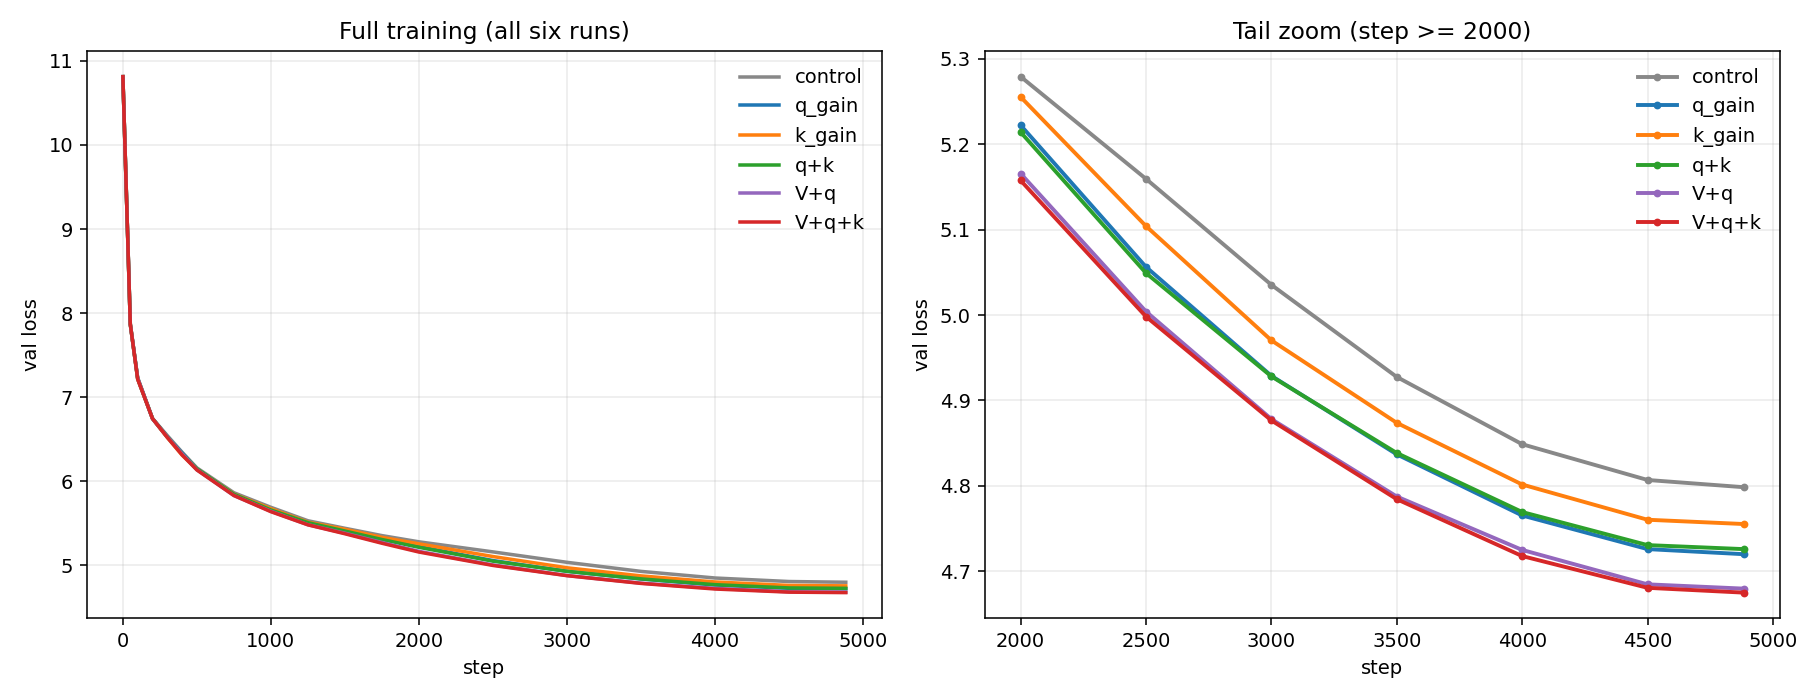
\includegraphics[width=0.8\linewidth]{loss_curves.png}
\caption{Validation loss over training. The per-head query gain stays below the
baseline for the full run.}
\label{fig:loss}
\end{figure}

\begin{figure}[h]
\centering
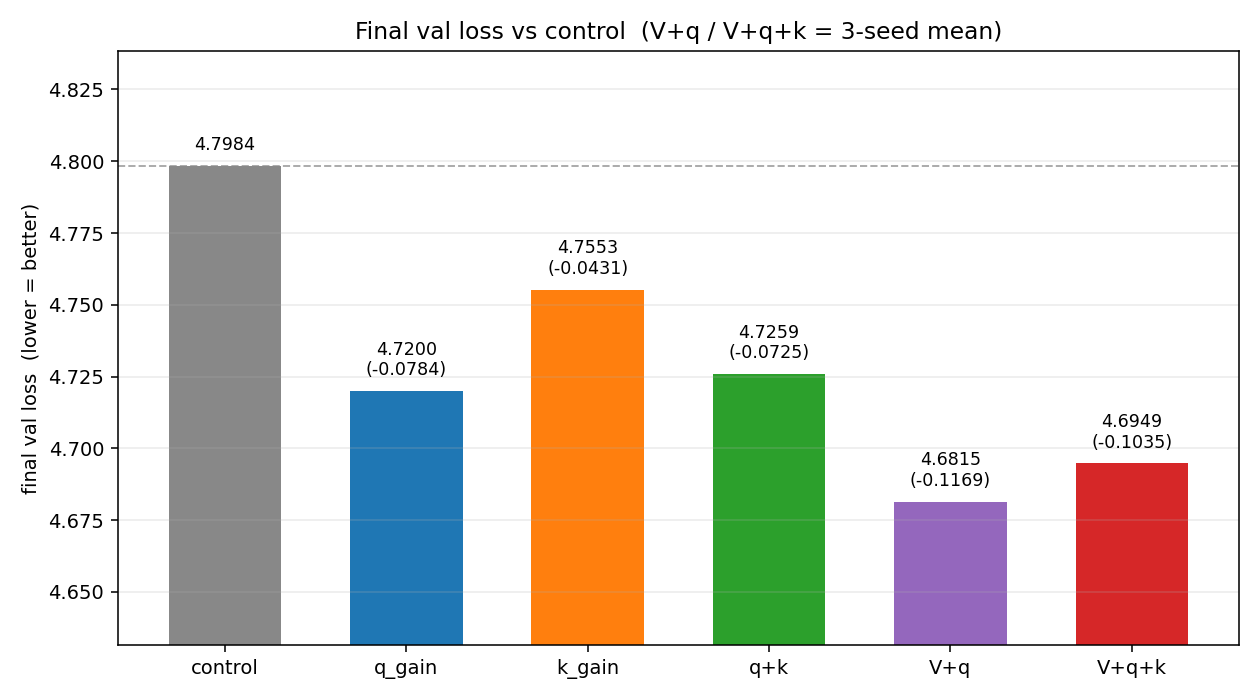
\includegraphics[width=0.6\linewidth]{final_val_bars.png}
\caption{Final validation loss. A $-0.078$ improvement for $144$ added scalars.}
\label{fig:bars}
\end{figure}

\section{Discussion}
The effect is small in absolute terms but large per parameter: $-0.078$
validation loss for $144$ scalars and no extra compute. The baseline pins every
head to a single sharpness; the gain lets each head pick its own, and the learned
values spread across heads rather than collapsing to zero. The mechanism is
orthogonal to architecture changes and can be applied to queries, keys, or both.

\section{Conclusion}
A single learnable sharpness scalar per head --- zero-initialized so the model
begins as the exact baseline --- is a cheap, safe knob that improves a small LLM's
validation loss at negligible cost. The lesson is not the magnitude of one number
but the principle: give attention an explicit control over its own sharpness, per
head, and let training decide.

\end{document}
